% Date : 10/03/2023
% Version : 4
% Auteur : ARN
% Relu : 
% Relecteur : Alexandre FAFIN

% ------------------------------------------------------------ %
% ----------------------  Fiche MAG03  ----------------------- %
% Thème : Champ magnétique
% Classes : MPSI, PCSI, PTSI
% ------------------------------------------------------------ %



% ======================================================= % 
% ============== Gestion de la compilation ============== %
% ======================================================= % 
\ifdefined\mainIsLoaded\else
\RequirePackage{import}
\subimport{../../}{_preambule_CdE_PC}
\begin{document}
\fi
% ======================================================= % 
% ======================================================= % 
	

% ======================================================= % 
% ===================== Couleurs ======================== %
% ======================================================= % 

% --------------------------------------------------------%
% La commande \couleurNBouCouleur prend deux paramètres :
% #1 est la couleur NB ; #2 est la couleur "en couleur"
%
\def\JRLblueF{\couleurNBouCouleur{gray}{blue!50}}
\def\JRLorange{\couleurNBouCouleur{gray}{orange}}
\def\JRLgreen{\couleurNBouCouleur{gray}{green!70!blue}}
\def\JRLred{\couleurNBouCouleur{gray}{red!90!green}}
\def\ECAred{\couleurNBouCouleur{darkgray}{\myCBDRed}}

% ======================================================= % 
% ======================================================= % 



% ============================================================================ %
%                            FICHE D'ENTRAÎNEMENT                              %
% ============================================================================ %
% ======================= Métadonnées sur la fiche =========================== %
\titreFicheEntrainement		{Champ magnétique}
\grandTheme					{Électromagnétisme}
\numeroFiche				{MAG03}
\uniqueID					{CBlNwAkVSb} % une chaîne de caractères (a-z, A-Z) aléatoire de 10 caractères.
\nombreColonnesReponses		{2} % 1, 2, 3, etc.
% ============================================================================ %

%%%%%%%%%%%%%%%%%%%%%%%%%%%%%%%%%%%%%%%%%%%%%%%%%%%%%%%%%%%%%%%%%%%%%%%%%%%%%%%%%%%%%%%%%%%%%%
\debutFicheEntrainement                                                                      %
%%%%%%%%%%%%%%%%%%%%%%%%%%%%%%%%%%%%%%%%%%%%%%%%%%%%%%%%%%%%%%%%%%%%%%%%%%%%%%%%%%%%%%%%%%%%%%

% --------------------------------------------------------------------- %
%                              Prérequis                                %
%                            (facultatif)                               %
% --------------------------------------------------------------------- %
% ================== Métadonnées sur le prérequis ===================== %
\avecPrerequis{Y} % Y ou N
% 
% ===================================================================== %

\begin{prerequis}
La force magnétique agissant sur une charge $q$, de vitesse $\vv{v}$, placée dans un champ magnétique $\vv{B}$ vaut $\vv{F_{\text{mag}}}= q \vv{v} \wedge \vv{B}$, où
$\vv{B}$ est un vecteur axial (ou pseudo-vecteur) dont l'unité est le tesla (noté $\si{\tesla}$).

\constantesUtiles
	\begin{listeConstantes}
		\item perméabilité magnétique du vide : $\mu_0=\SI{4\pi e-7}{T.m.A^{-1}}$
	\end{listeConstantes}
\end{prerequis}





% •••••••••••••••••••••••••••••••••••••••••••••••••••••••••••••••••••••••••••• %
% •••••••••••••••••••••••••••••••••••••••••••••••••••••••••••••••••••••••••••• %
\sectionFicheEntrainement{Pour commencer}
% •••••••••••••••••••••••••••••••••••••••••••••••••••••••••••••••••••••••••••• %
% •••••••••••••••••••••••••••••••••••••••••••••••••••••••••••••••••••••••••••• %



% ********************************************************************* %
%                           ENTRAÎNEMENT                                % 
% ********************************************************************* %
% ================ Métadonnées sur l'entraînement ===================== %

\titreEntrainementFacultatif	{À propos de la force magnétique}
\hauteurLargeurCadreReponse		{5mm}{1.8cm}
\dureeResolutionFacultative		{1} % 1, 2, 3 ou 4
\typeEntrainement				{QCM} % Newton ou QCM ou AN ou vide (exercice "normal")
\nombreColonnesQuestions		{2} % vide, 1, 2, 3, etc.
\avecPlusieursQuestions			{N} % Y ou N
\initialisationEntrainement
% ===================================================================== %

La force magnétique agissant sur une charge $q$ animée d'une vitesse $\vv{v}$ est  
$\vv{F_{\text{mag}}} = q \vv{v} \wedge \vv{B}$.

% =============================================================================== %
\debutEntrainement
% =============================================================================== %

% ^^^^^^^^^^^^^^^^^^^^^^^^^^^^^^^^^^^^^^ %
%               Question                 %
% ^^^^^^^^^^^^^^^^^^^^^^^^^^^^^^^^^^^^^^ %

\begin{enonce}
A-t-on toujours $\vv{F_{\text{mag}}} \perp \vv{v}$ ?
\end{enonce}

\reponse{oui}

% ************************************** %

% ^^^^^^^^^^^^^^^^^^^^^^^^^^^^^^^^^^^^^^ %
%               Question                 %
% ^^^^^^^^^^^^^^^^^^^^^^^^^^^^^^^^^^^^^^ %

\begin{enonce}
A-t-on toujours $\vv{F_{\text{mag}}} \perp \vv{B}$ ?
\end{enonce}

\reponse{oui}

% ************************************** %

% =============================================================================== %
\finEntrainement
% =============================================================================== %




% ********************************************************************* %
%                           ENTRAÎNEMENT                                % 
% ********************************************************************* %
% ================ Métadonnées sur l'entraînement 
% ===================== %

\titreEntrainementFacultatif	{Force magnétique connaissant le champ magnétique}
\hauteurLargeurCadreReponse		{8mm}{2cm}
\dureeResolutionFacultative		{1} % 1, 2, 3 ou 4
\typeEntrainement				{QCM} % Newton ou QCM ou AN ou vide (exercice "normal")
\basiqueEtTransversal			{Y}
\nombreColonnesQuestions		{1} % vide, 1, 2, 3, etc.
\avecPlusieursQuestions			{N} % Y ou N
\initialisationEntrainement
% ===================================================================== %

% mmmmmmmmmmmmmmmmmmmmmmmmmmmmmmmmmmmmmmmmmmmmmmmmmmmmmmmmm %
% 		  Insertion d'une image en regard d'un texte        %
% mmmmmmmmmmmmmmmmmmmmmmmmmmmmmmmmmmmmmmmmmmmmmmmmmmmmmmmmm %
% --------------------------------------------------------- %
\pourcentageDeLaPartieAGauche   {0.65}
% --------------------------------------------------------- %
%                                                           %
% -------------------- Partie à gauche -------------------- %
%                                                           %
                                \initialisationPartieGauche % 
%                                                           %
%                                                           %
Un électron de charge $-e$ possède un vecteur vitesse $\vv{v}=v_0 \vv{e_x}$ lorsqu'il est en $\ptO$. Il subit alors l'action d'un champ magnétique uniforme $\vv{B}=B_0(\vv{e_y} + \vv{e_z})$.

% --------------------------------------------------------- %
%                                                           %
% -------------------- Partie à droite -------------------- %
%                                                           %
                                \initialisationPartieDroite %
%                                                           %
%                                                           %
\begin{center}
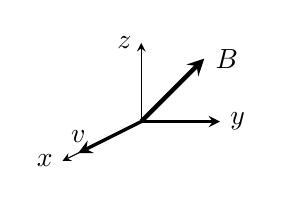
\begin{tikzpicture}[>=stealth, scale = 1]
\draw[->] (0,0)node[below]{$\ptO$} -- (-1,-0.5)node[left]{$x$};
\draw[->] (0,0)--(0,1)node[left]{$z$};
\draw[thick,->] (0,0)--(1,0)node[right]{$y$};
\draw[ultra thick, ->, \redOrBlack] (0,0)--(0.8,0.8)node[right]{$\vv{B}$};
\draw[very thick, ->, \blueOrDarkGray] (0,0)--(-0.8,-0.4)node[above]{$\vv{v}$};
\end{tikzpicture}
\end{center}
% --------------------------------------------------------- %
                               \finalisationDuPartageDePage %					
% --------------------------------------------------------- %

% =============================================================================== %
\debutEntrainement
% =============================================================================== %

% ^^^^^^^^^^^^^^^^^^^^^^^^^^^^^^^^^^^^^^ %
%               Question                 %
% ^^^^^^^^^^^^^^^^^^^^^^^^^^^^^^^^^^^^^^ %

\minusMedskip

\begin{enonce}
La force exercée sur l'électron en $\ptO$ vaut :
\begin{listeQCM2Colonnes}
		\item $\vv{F}=e v_0 B_0 (-\vv{e_y} - \vv{e_z})$
		\item $\vv{F}=e v_0 B_0 (\vv{e_y} + \vv{e_z})$
		\item $\vv{F}=e v_0 B_0 (-\vv{e_y} + \vv{e_z})$
		\item $\vv{F}=e v_0 B_0 (\vv{e_y} - \vv{e_z})$
	\end{listeQCM2Colonnes}
\end{enonce}

\reponse{$\reponseD{}$}

\begin{corrige} 
La force cherchée s'écrit $\vv{F}=-ev_{0}B_{0} ( \vv{e_x} \wedge \vv{e_y} + \vv{e_x} \wedge \vv{e_z} ) =ev_{0}B_{0} (\vv{e_y} -\vv{e_z} )$.
\end{corrige}

% ************************************** %

% =============================================================================== %
\finEntrainement
% =============================================================================== %


\minusMedskip


% ********************************************************************* %
%                           ENTRAÎNEMENT                                % 
% ********************************************************************* %
% ================ Métadonnées sur l'entraînement ===================== %

\titreEntrainementFacultatif	{Équilibre d'une boussole}
\hauteurLargeurCadreReponse		{7mm}{2cm}
\dureeResolutionFacultative		{2} % 1, 2, 3 ou 4
\typeEntrainement				{Newton} % Newton ou QCM ou AN ou vide (exercice "normal")
\nombreColonnesQuestions		{1} % vide, 1, 2, 3, etc.
\avecPlusieursQuestions			{Y} % Y ou N
\initialisationEntrainement
% ===================================================================== %


% mmmmmmmmmmmmmmmmmmmmmmmmmmmmmmmmmmmmmmmmmmmmmmmmmmmmmmmmm %
% 		  Insertion d'une image en regard d'un texte
% mmmmmmmmmmmmmmmmmmmmmmmmmmmmmmmmmmmmmmmmmmmmmmmmmmmmmmmmm %
% --------------------------------------------------------- %
\pourcentageDeLaPartieAGauche   {0.6}
% --------------------------------------------------------- %
%                                                           %
% -------------------- Partie à gauche -------------------- %
%                                                           %
                                \initialisationPartieGauche % 
%                                                           %
Une aiguille aimantée de centre $\ptO$ est libre de tourner sans frottements autour d'un axe vertical $(\ptO z)$. Elle s'oriente à l'équilibre suivant $\vv{B_H} = B_H \vv{e_x}$.% (composante horizontale du champ magnétique terrestre).\\

Un fil conducteur de grande longueur devant la taille de l'aiguille et placé à la distance $d = \SI{2}{cm}$ au dessus de $\ptO$, parallèlement à l'axe $(\ptO x)$.
Le champ magnétique créé en $\ptO$ par le fil vaut  
\[
\vv{B_{\text{fil}}}(\ptO)=\dfrac{\mu_0 I}{2 \pi d} \vv{e_y}.
\]

% --------------------------------------------------------- %
%                                                           %
% -------------------- Partie à droite -------------------- %
%                                                           %
                                \initialisationPartieDroite %
%                                                           %
\begin{center}
\def\scaleImage{0.75}
\subimport{_images/}{MAG03_boussole_ECA_v1.tex}
\end{center}
%
% --------------------------------------------------------- %
                               \finalisationDuPartageDePage %					
% --------------------------------------------------------- %


\smallskip

Lorsqu'un courant d'intensité $I=\SI{1.2}{A}$, circule dans ce fil dans le sens des $x$ croissants, 
la boussole retrouve une position d'équilibre en tournant d'un angle $\alpha=\ang{30}$ comme indiqué sur la figure.


\medskip

% =============================================================================== %
\debutEntrainement
% =============================================================================== %


% ^^^^^^^^^^^^^^^^^^^^^^^^^^^^^^^^^^^^^^ %
%               Question                 %
% ^^^^^^^^^^^^^^^^^^^^^^^^^^^^^^^^^^^^^^ %

\begin{enonce}
Exprimer $B_{H}$ en fonction de $\mu_{0}$,  $I$, $d$ et $\alpha$%en fonction des données.
\end{enonce}

\reponse{$\dfrac{\mu_{0} I}{2 \pi d \tan(\alpha)}$}

\begin{corrige}
À l'équilibre, la boussole s'oriente dans la direction du champ résultant
$\vv{B}(\ptO)=\vv{B_H}+\vv{B_{\text{fil}}}(\ptO)$. On a alors $\tan(\alpha)=\dfrac{B_{\text{fil}}}{B_H}$, d'où $B_{H}=\dfrac{\mu_0 I}{2 \pi d \tan(\alpha)}$.
\end{corrige}

% ************************************** %

% ^^^^^^^^^^^^^^^^^^^^^^^^^^^^^^^^^^^^^^ %
%               Question                 %
% ^^^^^^^^^^^^^^^^^^^^^^^^^^^^^^^^^^^^^^ %

\begin{enonce}
Donner la valeur numérique de $B_{H}$
\end{enonce}

\reponse{$\SI{20.8}{\micro T}$}

\begin{corrige} 
On calcule \minusSmallskip
\[
B_H
=\frac{\SI{4\pi e-7}{T.m.A^{-1}} \times \SI{1.2}{A}}{2\pi \times \SI{2e-2}{m} \times \tan(\ang{30})}
=\frac{\SI{ e-7}{T.m.A^{-1}} \times \SI{1.2}{A}}{\SI{1e-2}{m} \times \frac{1}{\sqrt{3}} }
=\sqrt{3}\times \SI{1,2  e-5}{T}=
\SI{20,8 e-6}{\si{\tesla}}.
\]
\end{corrige}

% ************************************** %

% =============================================================================== %
\finEntrainement
% =============================================================================== %


\newpage



% •••••••••••••••••••••••••••••••••••••••••••••••••••••••••••••••••••••••••••• %
% •••••••••••••••••••••••••••••••••••••••••••••••••••••••••••••••••••••••••••• %
\sectionFicheEntrainement{Calculs de flux magnétiques}
% •••••••••••••••••••••••••••••••••••••••••••••••••••••••••••••••••••••••••••• %
% •••••••••••••••••••••••••••••••••••••••••••••••••••••••••••••••••••••••••••• %

\medskip

Le flux $\Phi$ du champ magnétique à travers une surface $S$ reposant sur un contour orienté et fermé, s'écrit : 
\[
\Phi = \iint\limits_S \vv{B}\cdot \vv{\d{} S},
\]
où le vecteur $\vv{\d{} S}$ est orienté par la règle de Maxwell. 

On sait par ailleurs que $\vv{B}$ est un champ vectoriel à flux conservatif : le flux de $\vv{B}$ sortant de toute surface fermée est nul. 




% ********************************************************************* %
%                           ENTRAÎNEMENT                                % 
% ********************************************************************* %
% ================ Métadonnées sur l'entraînement ===================== %

\titreEntrainementFacultatif	{Flux d'un champ uniforme à travers une demi-sphère}
\hauteurLargeurCadreReponse		{8mm}{2cm}
\dureeResolutionFacultative		{2} % 1, 2, 3 ou 4
\typeEntrainement				{QCM} % Newton ou QCM ou AN ou vide (exercice "normal")
\nombreColonnesQuestions		{1} % vide, 1, 2, 3, etc.
\avecPlusieursQuestions			{N} % Y ou N
\initialisationEntrainement
% ===================================================================== %

% =============================================================================== %
\debutEntrainement
% =============================================================================== %

On considère la surface suivante, une demi-sphère de rayon $R$  et d'axe $(\ptO x)$.

\begin{center}
\subimport{_images/}{MAG03_flux_demi_sphere_CBD_v1.tex}
\end{center}

Combien vaut le flux du champ magnétique uniforme $\vv{B}=B \vv{e_x}$ à travers cette surface ?


\smallskip

% ^^^^^^^^^^^^^^^^^^^^^^^^^^^^^^^^^^^^^^ %
%               Question                 %
% ^^^^^^^^^^^^^^^^^^^^^^^^^^^^^^^^^^^^^^ %

\begin{enonce}
\begin{listeQCM3Colonnes}
		\item $\phi=0$
		\item $\phi=2B\pi R^2$
		\item $\phi=B\pi R^2$
\end{listeQCM3Colonnes}
\end{enonce}

\reponse{$\reponseC{}$}

\begin{corrige}
Au lieu d'exprimer le flux de $\vv{B}$ à travers la demi-sphère, il est plus simple de le calculer sur le disque qui s'appuie, comme la demi-sphère, sur la même circonférence de rayon $R$ (on utilise ici le fait que $\vv{B}$ est un champ vectoriel à flux conservatif).  
Sur le disque, on a $\vv{\d S}=\d{}S \vv{e_x}$. Ainsi $\phi=B \times S_{\text{disque}} = B \pi R^{2}$.
\end{corrige}

% ************************************** %

% =============================================================================== %
\finEntrainement
% =============================================================================== %






% ********************************************************************* %
%                           ENTRAÎNEMENT                                % 
% ********************************************************************* %
% ================ Métadonnées sur l'entraînement ===================== %

\titreEntrainementFacultatif	{Flux d'un champ non uniforme à travers un disque}
\hauteurLargeurCadreReponse		{11mm}{5cm}
\dureeResolutionFacultative		{2} % 1, 2, 3 ou 4
\typeEntrainement				{Newton} % Newton ou QCM ou AN ou vide (exercice "normal")
\nombreColonnesQuestions		{1} % vide, 1, 2, 3, etc.
\avecPlusieursQuestions			{N} % Y ou N
\initialisationEntrainement
% ===================================================================== %

% =============================================================================== %
\debutEntrainement
% =============================================================================== %



% mmmmmmmmmmmmmmmmmmmmmmmmmmmmmmmmmmmmmmmmmmmmmmmmmmmmmmmmm %
% 		  Insertion d'une image en regard d'un texte        %
% mmmmmmmmmmmmmmmmmmmmmmmmmmmmmmmmmmmmmmmmmmmmmmmmmmmmmmmmm %
% --------------------------------------------------------- %
\pourcentageDeLaPartieAGauche   {0.60}
% --------------------------------------------------------- %
%                                                           %
% -------------------- Partie à gauche -------------------- %
%                                                           %
                                \initialisationPartieGauche % 
%                                                           %
 
On considère un champ magnétique $\vv{B}$ défini par 
\[
\vv{B}(\ptM)=B_0 \left(1-\dfrac{r^2}{R^2} \right)\vv{e_x},
\]
 où $\ptM$ est repéré à l'aide des coordonnées cylindriques $r$, $\theta$ et $x$ Ainsi, $r$ est la distance du point à l'axe $(\ptO x)$.


% --------------------------------------------------------- %
%                                                           %
% -------------------- Partie à droite -------------------- %
%                                                           %
                                \initialisationPartieDroite %
% 
\begin{center}
\subimport{_images/}{MAG03_flux_disque_CBD_v1.tex}
\end{center}                                                          %
% 

% --------------------------------------------------------- %
                               \finalisationDuPartageDePage %					
% --------------------------------------------------------- %

\smallskip

On souhaite calculer le flux $\phi$ de ce champ à travers le disque de rayon $R$ et d'axe $(\ptO x)$  orienté comme indiqué sur la figure. Il est défini par
\[
\phi=\iint\limits_S \vv{B} \cdot \vv{\d{} S},
\]
où
$\vv{\d{} S}=\d{} S\,\vv{e_x}$ avec $\d S$ élément de surface du disque en un point $\ptM$ quelconque du disque.

\smallskip

On rappelle que l'expression de $\d S$ en coordonnées cylindriques est 
\[
\d S= r \cdot \d \theta\cdot \d r.
\]


% ^^^^^^^^^^^^^^^^^^^^^^^^^^^^^^^^^^^^^^ %
%               Question                 %
% ^^^^^^^^^^^^^^^^^^^^^^^^^^^^^^^^^^^^^^ %

\begin{enonce}
Exprimer $\phi$ en fonction de $R$ et $B_0$
\end{enonce}

\reponse{$\dfrac{ \pi}{2} B_{0} R^{2}$}

\begin{corrige}
On calcule \vspace{-4mm}
\[
\phi=\int\limits_{r=0}^R \, \int\limits_{\theta=0}^{2 \pi} \vv{B}\cdot\vv{e_x} \d r \times r \d \theta
=B_0 \times \left[ \pi R^{2}-\dfrac{2 \pi R^4}{4r^2} \right]
=\dfrac{\pi}{2}  R^2 B_0.
\]  
\end{corrige}

% ************************************** %

% =============================================================================== %
\finEntrainement
% =============================================================================== %


\newpage


% ********************************************************************* %
%                           ENTRAÎNEMENT                                % 
% ********************************************************************* %
% ================ Métadonnées sur l'entraînement ===================== %

\titreEntrainementFacultatif	{Flux à travers un cadre du champ créé par un fil}
\hauteurLargeurCadreReponse		{8mm}{4cm}
\dureeResolutionFacultative		{3} % 1, 2, 3 ou 4
\typeEntrainement				{Newton} % Newton ou QCM ou AN ou vide (exercice "normal")
\nombreColonnesQuestions		{1} % vide, 1, 2, 3, etc.
\avecPlusieursQuestions			{Y} % Y ou N
\initialisationEntrainement
% ===================================================================== %


% =============================================================================== %
\debutEntrainement
% =============================================================================== %

% mmmmmmmmmmmmmmmmmmmmmmmmmmmmmmmmmmmmmmmmmmmmmmmmmmmmmmmmm %
% 		  Insertion d'une image en regard d'un texte
% mmmmmmmmmmmmmmmmmmmmmmmmmmmmmmmmmmmmmmmmmmmmmmmmmmmmmmmmm %
% --------------------------------------------------------- %
\pourcentageDeLaPartieAGauche   {0.6}
% --------------------------------------------------------- %
%                                                           %
% -------------------- Partie à gauche -------------------- %
%                                                           %
                                \initialisationPartieGauche % 
%                                                           %
Considérons un fil rectiligne infiniment long suivant l'axe $(\ptO z)$, parcouru par un courant d'intensité $I$ circulant dans le sens des
$z$ croissants. Le champ magnétique créé par ce fil, en un point $\ptM$ à la distance $r$ de l'axe $(\ptO z)$, est : 
\[
\vv{B}(\ptM)=\dfrac{\mu_{0}I}{2\pi r} \vv{e_\theta}.
\]
%

% --------------------------------------------------------- %
%                                                           %
% -------------------- Partie à droite -------------------- %
%                                                           %
                                \initialisationPartieDroite %
%                                                           %
\begin{center}
\subimport{_images/}{MAG03_flux_cadre_carre_CBD_v1.tex}
\end{center}
%
% --------------------------------------------------------- %
                               \finalisationDuPartageDePage %					
% --------------------------------------------------------- %

Nous souhaitons calculer le flux $\phi$ de ce champ à travers le cadre carré de côté $a$ orienté comme indiqué sur la figure. Il est défini par
\[
\phi=\iint\limits_S \vv{B} \cdot \vv{\d{} S},
\]
où
$\vv{\d{} S}=\d{}S\,\vv{e_{\theta}}$ avec $\d{}S = \d{}r\cdot \d{}z$ élément de surface du cadre en un point $\ptM$ quelconque du cadre.



% ^^^^^^^^^^^^^^^^^^^^^^^^^^^^^^^^^^^^^^ %
%               Question                 %
% ^^^^^^^^^^^^^^^^^^^^^^^^^^^^^^^^^^^^^^ %

\begin{enonce}
Exprimer $\phi$ en fonction de $a$, $D$, $\mu_0$ et $I$
\end{enonce}

\reponse{$\dfrac{\mu_{0}Ia}{2\pi} \ln \left(\dfrac{D+a/2}{D-a/2} \right)$}

\begin{corrige}
On calcule \vspace{-4mm}
\[
\phi = 
\iintop_{\text{cadre}} \dfrac{\mu_{0}I}{2\pi r} \vv{e_\theta}\cdot \d{}S \vv{e_\theta}
= \dfrac{\mu_{0}I}{2\pi}\intop_{0}^{a} \d z \times \intop_{D-a/2}^{D+a/2} \dfrac{\d r}{r} 
= \dfrac{\mu_{0}Ia}{2\pi} \ln \left(\dfrac{D+a/2}{D-a/2} \right).
\]
\end{corrige}

% ************************************** %

% ^^^^^^^^^^^^^^^^^^^^^^^^^^^^^^^^^^^^^^ %
%               Question                 %
% ^^^^^^^^^^^^^^^^^^^^^^^^^^^^^^^^^^^^^^ %

\begin{enonce}
Donner un équivalent de $\phi$ si $a\ll D$.
\end{enonce}

\reponse{$\phi\approx\dfrac{\mu Ia^{2}}{2\pi D}$}

\begin{corrige}
On réécrit $\phi=\dfrac{\mu_{0}Ia}{2\pi}\left( \ln\left(1+\dfrac{a}{2D}\right)-\ln\left(1-\dfrac{a}{2D}\right)\right)$.
Un développement limité de $\ln\left(1\pm\varepsilon\right)$
à l'ordre 1 en $\varepsilon$ avec $\left|\varepsilon\right|\ll1$
donne alors : $\ln\left(1\pm\varepsilon\right)\approx\pm\varepsilon$. D'où $\phi\approx\dfrac{\mu Ia^{2}}{2\pi D}$.
\end{corrige}

% ************************************** %


% ^^^^^^^^^^^^^^^^^^^^^^^^^^^^^^^^^^^^^^ %
%               Question                 %
% ^^^^^^^^^^^^^^^^^^^^^^^^^^^^^^^^^^^^^^ %

\begin{enonce}
Que vaut $\phi$ si le cadre est situé dans un plan perpendiculaire à $(\ptO z)$ ?
\end{enonce}

\reponse{nul}

\begin{corrige}
Si le cadre est situé dans un plan perpendiculaire à $(\ptO z)$, on a
$\vv{\d S}=\d{}S\,\vv{e_z}$ et $\vv{B}\cdot\vv{\d S}=0$ : le flux est nul.
\end{corrige}

% ************************************** %

% =============================================================================== %
\finEntrainement
% =============================================================================== %






% •••••••••••••••••••••••••••••••••••••••••••••••••••••••••••••••••••••••••••• %
% •••••••••••••••••••••••••••••••••••••••••••••••••••••••••••••••••••••••••••• %
\sectionFicheEntrainement{Superposition de champs}
% •••••••••••••••••••••••••••••••••••••••••••••••••••••••••••••••••••••••••••• %
% •••••••••••••••••••••••••••••••••••••••••••••••••••••••••••••••••••••••••••• %




% ********************************************************************* %
%                           ENTRAÎNEMENT                                % 
% ********************************************************************* %
% ================ Métadonnées sur l'entraînement ===================== %

\titreEntrainementFacultatif	{Champ de deux aimants droits}
\hauteurLargeurCadreReponse		{8mm}{4cm}
\dureeResolutionFacultative		{2} % 1, 2, 3 ou 4
\typeEntrainement				{Newton} % Newton ou QCM ou AN ou vide (exercice "normal")
\basiqueEtTransversal			{Y}
\nombreColonnesQuestions		{1} % vide, 1, 2, 3, etc.
\avecPlusieursQuestions			{Y} % Y ou N
\initialisationEntrainement
% ===================================================================== %


% =============================================================================== %
\debutEntrainement
% =============================================================================== %

% mmmmmmmmmmmmmmmmmmmmmmmmmmmmmmmmmmmmmmmmmmmmmmmmmmmmmmmmm %
% 		  Insertion d'une image en regard d'un texte
% mmmmmmmmmmmmmmmmmmmmmmmmmmmmmmmmmmmmmmmmmmmmmmmmmmmmmmmmm %
% --------------------------------------------------------- %
\pourcentageDeLaPartieAGauche   {0.50}
% --------------------------------------------------------- %
%                                                           %
% -------------------- Partie à gauche -------------------- %
%                                                           %
                                \initialisationPartieGauche % 
%                                                           %
On approche le pôle Nord d'un aimant droit d'axe $\Delta$ du pôle Nord d'un aimant droit identique d'axe $(x'x)$.

On donne les champs créés par les aimants en $\ptO$ :

$\vv{B_1} = B_0 \vv{e_x}$ et $\vv{B_2} = B_0 \vv{e_\Delta}$ avec $B_0 = \SI{20}{mT}$. 
%
%
% --------------------------------------------------------- %
%                                                           %
% -------------------- Partie à droite -------------------- %
%                                                           %
                                \initialisationPartieDroite %
%                                                           %
\begin{center}
\subimport{_images/}{MAG03_aimant_ECA_v1.tex}
\end{center}
%
% --------------------------------------------------------- %
                               \finalisationDuPartageDePage %					
% --------------------------------------------------------- %

Le champ magnétique résultant de la superposition de $\vv{B_1}$ et $\vv{B_2} $ en $\ptO$ sera noté $\vv{B}(\ptO)$.
% ^^^^^^^^^^^^^^^^^^^^^^^^^^^^^^^^^^^^^^ %
%               Question                 %
% ^^^^^^^^^^^^^^^^^^^^^^^^^^^^^^^^^^^^^^ %

\begin{enonce}
Exprimer $\vv{B}(\ptO)$ dans la base $\left(\vv{e_x},\vv{e_y}\right)$, en fonction de $B_0$ et $\alpha$
\end{enonce}

\reponse{$B_0 \left(1+\cos(\alpha) \right) \vv{e_x} + B_0 \sin(\alpha) \vv{e_y}$}

\begin{corrige}
Le champ résultant en $\ptO$ s'écrit : $\vv{B}(\ptO)= \vv{B_1} + \vv{B_2}$ soit
$\vv{B}(\ptO)= B_0 \left ( 1+ \cos(\alpha) \right ) \vv{e_x} + B_0 \sin(\alpha)\vv{e_y}$.
\end{corrige}

% ^^^^^^^^^^^^^^^^^^^^^^^^^^^^^^^^^^^^^^ %
%               Question                 %
% ^^^^^^^^^^^^^^^^^^^^^^^^^^^^^^^^^^^^^^ %

\begin{enonce}
Exprimer la norme $B(\ptO)$ de $\vv{B}(\ptO)$, en fonction de $B_0$ et $\cos(\alpha)$ 
\end{enonce}

\reponse{$B_0 \sqrt{2\left(1 + \cos(\alpha)\right)}$}

\begin{corrige} 
On a $B(\ptO) = B_0 \sqrt{(1+\cos(\alpha))^2 + \sin^2(\alpha)}$.
Donc, $B(\ptO) = B_0 \sqrt{2\left(1+\cos(\alpha)\right)}$.
\end{corrige}


% ^^^^^^^^^^^^^^^^^^^^^^^^^^^^^^^^^^^^^^ %
%               Question                 %
% ^^^^^^^^^^^^^^^^^^^^^^^^^^^^^^^^^^^^^^ %

\begin{enonce}
Calculer $B(\ptO)$ pour $\alpha = \ang{60}$
\end{enonce}

\reponse{$\SI{34.6}{mT}$}

\begin{corrige}
On a $B(\ptO)= 20 \sqrt{3} \, \si{m \tesla}$ et donc $B(\ptO)=\SI{34.6}{mT}$.
\end{corrige}

% =============================================================================== %
\finEntrainement
% =============================================================================== %



\newpage


% ********************************************************************* %
%                           ENTRAÎNEMENT                                % 
% ********************************************************************* %
% ================ Métadonnées sur l'entraînement ===================== %

\titreEntrainementFacultatif	{Champ magnétique créé par deux fils}
\hauteurLargeurCadreReponse		{8mm}{5cm}
\dureeResolutionFacultative		{3} % 1, 2, 3 ou 4
\typeEntrainement				{Newton} % Newton ou QCM ou AN ou vide (exercice "normal")
\basiqueEtTransversal			{Y}
\nombreColonnesQuestions		{1} % vide, 1, 2, 3, etc.
\avecPlusieursQuestions			{Y} % Y ou N
\initialisationEntrainement
% ===================================================================== %

% =============================================================================== %
\debutEntrainement
% =============================================================================== %

%% mmmmmmmmmmmmmmmmmmmmmmmmmmmmmmmmmmmmmmmmmmmmmmmmmmmmmmmmm %
%% 		  Insertion d'une image en regard d'un texte
%% mmmmmmmmmmmmmmmmmmmmmmmmmmmmmmmmmmmmmmmmmmmmmmmmmmmmmmmmm %
%% --------------------------------------------------------- %
%\pourcentageDeLaPartieAGauche   {0.525}
%% --------------------------------------------------------- %
%%                                                           %
%% -------------------- Partie à gauche -------------------- %
%%                                                           %
%                                \initialisationPartieGauche % 
%%                                                           %
Deux fils colinéaires à l'axe $(\ptO z)$ et parcourus par un courant d'intensité $I$ coupent le plan $(x \ptO y)$ respectivement en $\ptO_1$ et $\ptO_2$, comme représenté ci-dessous :

\begin{center}
\subimport{_images/}{MAG03_deux_autres_fils_CBD_v1.tex}
\end{center}

Ces fils passant par $\ptO_1$ et par $\ptO_2$ créent, au point $\ptD(0,y)$, respectivement, les champs $\vv{B_1}$ et $\vv{B_2}$ vérfiant
\[
\vv{B_1} = B_0\, \vv{e_1} \qquad \text{et} \qquad \vv{B_2} = B_0\, \vv{e_2}.
\]

On donne $B_0=\dfrac{\mu_0 I}{2 \pi d}$,
où $d$ est la distance commune de $\ptD$ aux points $\ptO_1$ et $\ptO_2$.

Le vecteur $\vv{e_1}$ est un vecteur unitaire orthogonal à la droite $(\ptO_1\ptD)$ ; de même pour $\vv{e_2}$.

%% --------------------------.------------------------------- %
%%                                                           %
%% -------------------- Partie à droite -------------------- %
%%                                                           %
%                                \initialisationPartieDroite %
%%                                                           %
%\begin{center}
%\begin{tikzpicture}[>=stealth]
%\draw[->] (-2.5,0)--(2,0)node[right]{$x$};
%\draw[->] (0,-1)--(0,3)node[left]{$y$};
%\draw (0,0)node{$\bullet$}node[above right]{$\ptO$};
%\draw (-0.75,0) node[above left]{$\ptO_{1}$};
%\draw (0.75,0) node[above right]{$\ptO_{2}$};
%\draw (0,2)node{$\bullet$} node[above right]{$\ptD$};
%\draw[<->] (0,-0.5)--(-0.75,-0.5)node[above, midway]{$a$};
%\draw[<->] (0,-0.5)--(0.75,-0.5)node[above, midway]{$a$};
%\draw[dashed] (-0.75,0)--(-0.75,-0.5) (0.75,0)--(0.75,-0.5);
%\draw[dashed] (-0.75,0)--(0,2)node[left, midway]{$d$} (0.75,0)--(0,2)node[right, midway]{$d$};
%\draw[very thick, red, ->] (0,2)--(-1.75,2.75)node[black, left]{$\vv{B_1}$};
%\draw[very thick, red, ->] (0,2)--(-1.75,1.25)node[black, left]{$\vv{B_2}$};
%\draw[->] (-0.25,0) arc(0:53:0.75)node[right, midway]{$\theta$};
%\draw[ultra thick, \blueOrBlack,->] (0,2)--(-1.2,2.5) node[black, above]{$\vv{e_1}$};
%\draw[ultra thick, \blueOrBlack,->] (0,2)--(-1.2,1.5) node[black, below]{$\vv{e_2}$};
%\draw (-0.15,1.9)node[rotate=-25]{$\Box$};
%\draw (0.15,1.9)node[rotate=25]{$\Box$};
%\draw[dashed] (0,2)--(1.75,2.75);
%\draw (0.75,0)node{$\odot$};
%\draw (-0.75,0)node{$\odot$};
%\end{tikzpicture}
%\end{center}
%%
%% --------------------------------------------------------- %
%                               \finalisationDuPartageDePage %					
%% --------------------------------------------------------- %

\smallskip

Le champ magnétique résultant de la superposition de $\vv{B_1}$ et $\vv{B_2} $ en $\ptD$ sera noté $\vv{B_{\text{tot}}}$.

\smallskip


% ^^^^^^^^^^^^^^^^^^^^^^^^^^^^^^^^^^^^^^ %
%               Question                 %
% ^^^^^^^^^^^^^^^^^^^^^^^^^^^^^^^^^^^^^^ %

\begin{enonce}
Exprimer $d$ en fonction de $a$ et $\theta$
\end{enonce}

\reponse{$\dfrac{a}{\cos(\theta)}$}

\begin{corrige}
On a $\cos(\theta) = \dfrac{a}{d}$ d'où le résultat.
\end{corrige}

% ^^^^^^^^^^^^^^^^^^^^^^^^^^^^^^^^^^^^^^ %
%               Question                 %
% ^^^^^^^^^^^^^^^^^^^^^^^^^^^^^^^^^^^^^^ %

\begin{enonce}
Exprimer $\vv{e_1}$ dans la base $(\vv{e_x}, \vv{e_y})$
\end{enonce}

\reponse{$-\sin(\theta)\vv{e_x} + \cos(\theta)\vv{e_y}$}

\begin{corrige}
L'angle orienté $\theta$, entre l'horizontale $(\ptO x)$ et la demi-droite $[\ptO_1  \ptD)$ se retrouve entre la verticale $(\ptO y)$ et la perpendiculaire à $[\ptO_1 \ptD)$, c'est-à-dire la direction du vecteur $\vv{e_1}$.
On a donc $\vv{e_1}=-\sin(\theta)\vv{e_x} + \cos(\theta)\vv{e_y}$.
\end{corrige}

% ^^^^^^^^^^^^^^^^^^^^^^^^^^^^^^^^^^^^^^ %
%               Question                 %
% ^^^^^^^^^^^^^^^^^^^^^^^^^^^^^^^^^^^^^^ %

\begin{enonce}
Exprimer $\vv{e_2}$ dans la base $(\vv{e_x}, \vv{e_y})$
\end{enonce}

\reponse{$-\sin(\theta)\vv{e_x} - \cos(\theta)\vv{e_y}$}

\begin{corrige}
Si on note $\beta$ l'angle que fait $\vv{e_2}$ avec la verticale descendante ($-\ptO y$), on a $\beta + \dfrac{\pi}{2} - \theta = \dfrac{\pi}{2}$, donc $\beta =\theta$. On a donc $\vv{e_2}=-\sin(\theta)\vv{e_x} - \cos(\theta)\vv{e_y}$.
\end{corrige}

% ^^^^^^^^^^^^^^^^^^^^^^^^^^^^^^^^^^^^^^ %
%               Question                 %
% ^^^^^^^^^^^^^^^^^^^^^^^^^^^^^^^^^^^^^^ %

\begin{enonce}
Exprimer $\vv{B_{\text{tot}}}$ dans la base $(\vv{e_x}, \vv{e_y})$ en fonction de $B_0$ et $\theta$
\end{enonce}

\reponse{$-2B_0 \sin(\theta) \vv{e_x}$}

\begin{corrige}
Le champ résultant en $\ptD$ s'écrit $\vv{B_{\text{tot}}}=B_0(\vv{e_1}+\vv{e_2})$. En utilisant les résultats précédents, on trouve $\vv{B_{\text{tot}}}=-2B_0 \sin(\theta)\vv{e_x}$.
\end{corrige}



% =============================================================================== %
\pauseEntrainement
% =============================================================================== %

\bigskip

Le champ $\vv{B_{\text{tot}}}$ peut se mettre sous la forme suivante :
\[
\vv{B_{\text{tot}}}=\dfrac{\mu_0 I}{\pi}f(y) \vv{e_x}.
\]
 
% =============================================================================== %
\repriseEntrainement
% =============================================================================== %


% ^^^^^^^^^^^^^^^^^^^^^^^^^^^^^^^^^^^^^^ %
%               Question                 %
% ^^^^^^^^^^^^^^^^^^^^^^^^^^^^^^^^^^^^^^ %
\begin{enonce}
Expliciter la fonction $f(y)$ en fonction de $a$ et $y$.
\end{enonce}

\reponse{$-\dfrac{y}{a^2 + y^2}$}

\begin{corrige} 
On a $\sin(\theta)=\dfrac{y}{d}$. De plus, dans le triangle rectangle $\left(\ptO\, \ptO_1\, \ptD\right) $, on a   $d^2=a^2+y^2$. 

Ainsi, 
$\vv{B_{\text{tot}}}=-\dfrac{\mu_0 I}{\pi}\dfrac{y}{a^2 + y^2},\vv{e_x}$.
Par conséquent, on a $f(y)=-\dfrac{y}{a^2 + y^2}$.
\end{corrige}


% ^^^^^^^^^^^^^^^^^^^^^^^^^^^^^^^^^^^^^^ %
%               Question                 %
% ^^^^^^^^^^^^^^^^^^^^^^^^^^^^^^^^^^^^^^ %

\begin{enonce}
Pour quelles valeurs de $y$, $\vaB{f(y)}$ est-elle maximale ?
\end{enonce}

\reponse{en $y = \pm a$}

\begin{corrige}
On calcule $f'(y)=\dfrac{-(a^2+y^2)+y\times 2y}{(a^2 + y^2)^2} = \dfrac{y^2-a^2}{(a^2+y^2)^2}$. La fonction
$f'$ s'annule pour $|y| \to \infty$, qui renvoie $\lim \limits_{|y| \to \infty} f(y) = 0$ et pour $|y|=a$ qui donne $\big|f(\pm a)\big|=\dfrac{1}{2a}$ : c'est le maximum recherché.
\end{corrige}


% =============================================================================== %
\finEntrainement
% =============================================================================== %




\newpage


% •••••••••••••••••••••••••••••••••••••••••••••••••••••••••••••••••••••••••••• %
% •••••••••••••••••••••••••••••••••••••••••••••••••••••••••••••••••••••••••••• %
\sectionFicheEntrainement{Champs magnétiques créés par des courants}
% •••••••••••••••••••••••••••••••••••••••••••••••••••••••••••••••••••••••••••• %
% •••••••••••••••••••••••••••••••••••••••••••••••••••••••••••••••••••••••••••• %





% ********************************************************************* %
%                           ENTRAÎNEMENT                                % 
% ********************************************************************* %
% ================ Métadonnées sur l'entraînement ===================== %

\titreEntrainementFacultatif	{N fils sur un cylindre}
\hauteurLargeurCadreReponse		{8mm}{2cm}
\dureeResolutionFacultative		{1} % 1, 2, 3 ou 4
\typeEntrainement				{QCM} % Newton ou QCM ou AN ou vide (exercice "normal")
\nombreColonnesQuestions		{1} % vide, 1, 2, 3, etc.
\avecPlusieursQuestions			{Y} % Y ou N
\initialisationEntrainement
% ===================================================================== %

% =============================================================================== %
\debutEntrainement
% =============================================================================== %


% mmmmmmmmmmmmmmmmmmmmmmmmmmmmmmmmmmmmmmmmmmmmmmmmmmmmmmmmm %
% 		  Insertion d'une image en regard d'un texte
% mmmmmmmmmmmmmmmmmmmmmmmmmmmmmmmmmmmmmmmmmmmmmmmmmmmmmmmmm %
% --------------------------------------------------------- %
\pourcentageDeLaPartieAGauche   {0.55}
% --------------------------------------------------------- %
%                                                           %
% -------------------- Partie à gauche -------------------- %
%                                                           %
                                \initialisationPartieGauche % 
%                                                           %
On considère $N$ fils rectilignes ($N\gg1$) infiniment longs, uniformément répartis
sur un cylindre de centre $\ptO$, de rayon $a$ et d'axe $(\ptO z)$. Ces fils
sont parcourus par le même courant circulant dans le même sens.

Soit un point $\ptM$ à la distance $r$ de $\ptO$.
%
% --------------------------------------------------------- %
%                                                           %
% -------------------- Partie à droite -------------------- %
%                                                           %
                                \initialisationPartieDroite %

\begin{center}
\subimport{_images/}{MAG03_N_fils_CBD_v1.tex}
\end{center}                                         

% 
% --------------------------------------------------------- %
                               \finalisationDuPartageDePage %					
% --------------------------------------------------------- %

% ^^^^^^^^^^^^^^^^^^^^^^^^^^^^^^^^^^^^^^ %
%               Question                 %
% ^^^^^^^^^^^^^^^^^^^^^^^^^^^^^^^^^^^^^^ %

\begin{enonce}
Pour la distribution des courants, le plan $(\ptM,\vv{e_r},\vv{e_z})$ est un plan :
	\begin{listeQCM2Colonnes}
		\item de symétrie
		\item d'antisymétrie
		\item ni de symétrie, ni d'antisymétrie
	\end{listeQCM2Colonnes}
\end{enonce}

\reponse{$\reponseA{}$}

\begin{corrige}
Le plan $(M, \vv{e_r}, \vv{e_z})$ est un plan de symétrie qui laisse $\ptM$ invariant ainsi que la distribution des courants car si $N\gg1$, chaque fil aura son symétrique, le courant circulant dans le même sens dans les deux fils symétriques.
\end{corrige}


% ^^^^^^^^^^^^^^^^^^^^^^^^^^^^^^^^^^^^^^ %
%               Question                 %
% ^^^^^^^^^^^^^^^^^^^^^^^^^^^^^^^^^^^^^^ %

\begin{enonce}
Le champ magnétique en $\ptM$ est alors :
	\begin{listeQCM2Colonnes}
		\item dirigé selon $\vv{e_r}$
		\item dirigé selon $\vv{e_\theta}$
		\item dirigé selon $\vv{e_z}$
	\end{listeQCM2Colonnes}
\end{enonce}


\reponse{$\reponseB{}$}

\begin{corrige} 
Le vecteur $\vv{B}$ vecteur axial est perpendiculaire à tout plan de symétrie de ses sources, donc $\vv{B}(\ptM)$ est dirigé selon $\vv{e_\theta}$.
\end{corrige}

% =============================================================================== %
\finEntrainement
% =============================================================================== %



% ********************************************************************* %
%                           ENTRAÎNEMENT                                % 
% ********************************************************************* %
% ================ Métadonnées sur l'entraînement ===================== %

\titreEntrainementFacultatif	{Champ créé par deux fils parallèles}
\hauteurLargeurCadreReponse		{8mm}{2cm}
\dureeResolutionFacultative		{2} % 1, 2, 3 ou 4
\typeEntrainement				{QCM} % Newton ou QCM ou AN ou vide (exercice "normal")
\nombreColonnesQuestions		{1} % vide, 1, 2, 3, etc.
\avecPlusieursQuestions			{Y} % Y ou N
\initialisationEntrainement
% ===================================================================== %


% =============================================================================== %
\debutEntrainement
% =============================================================================== %

% mmmmmmmmmmmmmmmmmmmmmmmmmmmmmmmmmmmmmmmmmmmmmmmmmmmmmmmmm %
% 		  Insertion d'une image en regard d'un texte
% mmmmmmmmmmmmmmmmmmmmmmmmmmmmmmmmmmmmmmmmmmmmmmmmmmmmmmmmm %
% --------------------------------------------------------- %
\pourcentageDeLaPartieAGauche   {0.50}
% --------------------------------------------------------- %
%                                                           %
% -------------------- Partie à gauche -------------------- %
%                                                           %
                                \initialisationPartieGauche % 
%                                                           %
On considère deux fils conducteurs infinis parallèles à l'axe $(\ptO z)$,
distants de $2a$ et parcourus par des courants de même intensité $I$ circulant en sens inverse.


% --------------------------------------------------------- %
%                                                           %
% -------------------- Partie à droite -------------------- %
%                                                           %
                                \initialisationPartieDroite %
% 
\begin{center}
\subimport{_images/}{MAG03_deux_fils_CBD_v1.tex}
\end{center}                                                          %
% 
% --------------------------------------------------------- %
                               \finalisationDuPartageDePage %					
% --------------------------------------------------------- %

% ^^^^^^^^^^^^^^^^^^^^^^^^^^^^^^^^^^^^^^ %
%               Question                 %
% ^^^^^^^^^^^^^^^^^^^^^^^^^^^^^^^^^^^^^^ %
\begin{enonce}
Lequel de ces trois plans est plan de symétrie pour la distribution des courants ?
	\begin{listeQCM3Colonnes}
		\item le plan $(x \ptO y)$
		\item le plan $(y \ptO z)$
		\item le plan $(x \ptO z)$
	\end{listeQCM3Colonnes}
\bigskip
\end{enonce}

\reponse{$\reponseC{}$}

\begin{corrige}
Dans une symétrie par rapport au plan $(x \ptO y)$, les fils restent inchangés mais les courants sont inversés  : c'est donc un plan d'antisymétrie.

Dans une symétrie par rapport au plan $(y \ptO z)$, on permute les fils de gauche et de droite, les courants circulant dans le sens inverse de la situation initiale : il s'agit ici encore, d'un plan d'antisymétrie.

Seul, le plan $(x \ptO z)$ laisse les fils inchangés ainsi que les sens des courants : c'est donc bien un plan de symétrie pour la distribution des courants. 
\end{corrige}

% ************************************** %


% ^^^^^^^^^^^^^^^^^^^^^^^^^^^^^^^^^^^^^^ %
%               Question                 %
% ^^^^^^^^^^^^^^^^^^^^^^^^^^^^^^^^^^^^^^ %

\begin{enonce}
L'analyse des symétries permet de dire qu'en un point $\ptA$ de l'axe $(\ptO x)$, le champ $\vv{B}(\ptA)$ est : 
\begin{listeQCM3Colonnes}
		\item parallèle à $(\ptO x)$
		\item parallèle à $(\ptO y)$
		\item parallèle à $(\ptO z)$
\end{listeQCM3Colonnes}
\bigskip
\end{enonce}

\reponse{$\reponseB{}$}

\begin{corrige}
Pour le point $\ptA$ sur l'axe $(\ptO x)$, le plan $(x \ptO y)$ est un plan de symétrie pour la distribution des courants et laisse $\ptA$ invariant. Le vecteur champ magnétique, vecteur axial, est perpendiculaire à tout plan de symétrie, donc on a $\vv{B}(\ptA) \perp (x \ptO z)$. Donc, $\vv{B}(\ptA)$ est parallèle à  $(\ptO y)$. 
\end{corrige}

% ************************************** %


% ^^^^^^^^^^^^^^^^^^^^^^^^^^^^^^^^^^^^^^ %
%               Question                 %
% ^^^^^^^^^^^^^^^^^^^^^^^^^^^^^^^^^^^^^^ %

\begin{enonce}
L'analyse des symétries permet de dire qu'en un point $\ptD$ de l'axe $(\ptO y)$, le champ $\vv{B}(\ptD)$ est : 
\begin{listeQCM3Colonnes}
		\item parallèle à $(\ptO x)$
		\item parallèle à $(\ptO y)$
		\item parallèle à $(\ptO z)$
\end{listeQCM3Colonnes}
\bigskip
\end{enonce}

\reponse{$\reponseB{}$}

\begin{corrige}
Pour le point $\ptD$ sur l'axe $(\ptO y)$, les plans $(x \ptO y)$ et $(y \ptO z)$ sont des plans d'antisymétrie pour la distribution des courants et laissent $\ptD$ invariant. Le vecteur champ magnétique, vecteur axial, est contenu dans tout plan d'antisymétrie, donc $\vv{B_{\text{tot}}} \in (x \ptO y)\cap (y \ptO z)$, soit $\vv{B_{\text{tot}}}$ est parallèle à  $(\ptO y)$. 
\end{corrige}


% =============================================================================== %
\finEntrainement
% =============================================================================== %



\newpage



% ********************************************************************* %
%                           ENTRAÎNEMENT                                % 
% ********************************************************************* %
% ================ Métadonnées sur l'entraînement ===================== %

\titreEntrainementFacultatif	{Champ créé par une spire circulaire}
\hauteurLargeurCadreReponse		{8mm}{2cm}
\dureeResolutionFacultative		{1} % 1, 2, 3 ou 4
\typeEntrainement				{QCM} % Newton ou QCM ou AN ou vide (exercice "normal")
\nombreColonnesQuestions		{1} % vide, 1, 2, 3, etc.
\avecPlusieursQuestions			{Y} % Y ou N
\initialisationEntrainement
% ===================================================================== %


% mmmmmmmmmmmmmmmmmmmmmmmmmmmmmmmmmmmmmmmmmmmmmmmmmmmmmmmmm %
% 		  Insertion d'une image en regard d'un texte
% mmmmmmmmmmmmmmmmmmmmmmmmmmmmmmmmmmmmmmmmmmmmmmmmmmmmmmmmm %
% --------------------------------------------------------- %
\pourcentageDeLaPartieAGauche   {0.55}
% --------------------------------------------------------- %
%                                                           %
% -------------------- Partie à gauche -------------------- %
%                                                           %
                                \initialisationPartieGauche % 
%                                                           %
On considère une spire circulaire de centre $\ptO$, d'axe $(\ptO z)$ et de rayon $R$, parcourue par un courant d'intensité $I>0$ constante circulant dans le sens indiqué sur la figure.

On cherche la direction du champ $\vv{B}$ créé par la spire en un point $\ptM$ de l'axe $(\ptO z)$, puis en $\ptN$ à la distance $r$ de $\ptM$.

% --------------------------------------------------------- %
%                                                           %
% -------------------- Partie à droite -------------------- %
%                                                           %
                                \initialisationPartieDroite %
% 
\begin{center}
\subimport{_images/}{MAG03_champ_cree_spire_circulaire_CBD_v1.tex}
\end{center}                                                          
%
% 
% --------------------------------------------------------- %
                               \finalisationDuPartageDePage %					
% --------------------------------------------------------- %


% =============================================================================== %
\debutEntrainement
% =============================================================================== %

% ^^^^^^^^^^^^^^^^^^^^^^^^^^^^^^^^^^^^^^ %
%               Question                 %
% ^^^^^^^^^^^^^^^^^^^^^^^^^^^^^^^^^^^^^^ %
\begin{enonce}
En un point M de l'axe $(\ptO z)$, le champ créé par la spire est
	\begin{listeQCM3Colonnes}
		\item colinéaire à $\vv{e_r}$
		\item colinéaire à $\vv{e_\theta}$
		\item colinéaire à $\vv{e_z}$
	\end{listeQCM3Colonnes}
\bigskip
\end{enonce}

\reponse{$\reponseC{}$}

\begin{corrigeNewpage}
Tout plan qui contient le point $\ptM$ et l'axe $(\ptO z)$ est plan d'antisymétrie pour la distribution des courants et laisse $\ptM$ invariant. Le vecteur $\vv{B}(\ptM)$, vecteur axial est contenu dans tous ces plans d'antisymétrie. Par conséquent, $\vv{B}(\ptM)$ est colinéaire à $(\ptO z)$.
\end{corrigeNewpage}

% ************************************** %


% ^^^^^^^^^^^^^^^^^^^^^^^^^^^^^^^^^^^^^^ %
%               Question                 %
% ^^^^^^^^^^^^^^^^^^^^^^^^^^^^^^^^^^^^^^ %

\begin{enonce}
L'analyse des symétries permet de dire qu'en $\ptN$, le champ $\vv{B}(\ptN)$ est contenu dans le plan : 
	\begin{listeQCM3Colonnes}
		\item $(\ptM, \vv{e_r}, \vv{e_\theta})$
		\item $(\ptM, \vv{e_\theta}, \vv{e_z})$
		\item $(\ptM, \vv{e_r}, \vv{e_z})$
	\end{listeQCM3Colonnes}
\bigskip
\end{enonce}

\reponse{$\reponseC{}$ }

\begin{corrige}
Le plan $(\ptM, \vv{e_r}, \vv{e_z})$ est un plan d'antisymétrie pour la distribution des courants et laisse le point $\ptN$ invariant. Le vecteur champ magnétique, vecteur axial, est contenu dans tout plan d'antisymétrie, donc on a $\vv{B}(\ptN) \in (\ptM, \vv{e_r}, \vv{e_z})$. 
\end{corrige}

% ************************************** %

% =============================================================================== %
\finEntrainement
% =============================================================================== %





% ********************************************************************* %
%                           ENTRAÎNEMENT                                % 
% ********************************************************************* %
% ================ Métadonnées sur l'entraînement ===================== %

\titreEntrainementFacultatif	{Champ créé sur l'axe par une spire circulaire}
\hauteurLargeurCadreReponse		{8mm}{5cm}
\dureeResolutionFacultative		{2} % 1, 2, 3 ou 4
\typeEntrainement				{Newton} % Newton ou QCM ou AN ou vide (exercice "normal")
\basiqueEtTransversal			{Y}
\nombreColonnesQuestions		{1} % vide, 1, 2, 3, etc.
\avecPlusieursQuestions			{Y} % Y ou N
\initialisationEntrainement
% ===================================================================== %

{\itshape On reprend la spire circulaire de l'entraînement précédent.}

Le champ magnétique créé par cette spire en $\ptM (0,0,z)$ s'écrit : 
\[
\vv{B_{\text{axe}}}(\ptM)=\dfrac{\mu_0 I}{2R}\sin^3(\alpha)\vv{e_z},
\] 
où $\alpha$ est l'angle orienté dans le sens horaire sous lequel $\ptM$ voit le rayon de la spire.


Le vecteur $\vv{B_{\text{axe}}}(\ptM)$ peut également s'écrire en fonction de $z$. Il prendra alors la forme suivante : 
 \[
 \vv{B_{\text{axe}}}(\ptM)=\dfrac{\mu_0 I}{2R}f(z)\vv{e_z}.
 \]

% =============================================================================== %
\debutEntrainement
% =============================================================================== %


% ^^^^^^^^^^^^^^^^^^^^^^^^^^^^^^^^^^^^^^ %
%               Question                 %
% ^^^^^^^^^^^^^^^^^^^^^^^^^^^^^^^^^^^^^^ %

\begin{enonce}
Exprimer $\sin(\alpha)$ en fonction de $z$ et de $R$
\end{enonce}

\reponse{$\dfrac{R}{\sqrt{R^2+z^2}}$}

%\begin{corrige}
%\end{corrige}

% ************************************** %



% ^^^^^^^^^^^^^^^^^^^^^^^^^^^^^^^^^^^^^^ %
%               Question                 %
% ^^^^^^^^^^^^^^^^^^^^^^^^^^^^^^^^^^^^^^ %

\begin{enonce}
Exprimer $f(z)$ en fonction de $z$ et de $R$ 
\end{enonce}

\reponse{$\dfrac{R^3}{(\sqrt{R^2+z^2})^3}$}

\begin{corrige}
On a $B_0 f(z)= B_0 \sin^3(\alpha)$, ce qui donne $f(z)=\dfrac{R^3}{\left(\sqrt{R^2+z^2}\right)^3}$.
\end{corrige}

% ************************************** %


% =============================================================================== %
\pauseEntrainement
% =============================================================================== %


\bigskip

On note $B_1$ l'intensité du champ  $\vv{B_{\text{axe}}}(\ptM)$ quand $z=R$.


% =============================================================================== %
\repriseEntrainement
% =============================================================================== %




% ^^^^^^^^^^^^^^^^^^^^^^^^^^^^^^^^^^^^^^ %
%               Question                 %
% ^^^^^^^^^^^^^^^^^^^^^^^^^^^^^^^^^^^^^^ %

\begin{enonce}
Exprimer $B_1$ en fonction de $\mu_0$, $I$ et $R$
\end{enonce}

\reponse{$\frac{\mu_0I}{4\sqrt{2}\,R}$}

\begin{corrige}
Remplaçons $z$ par $R$ dans l'expression de $B_\text{axe}$. On trouve $B_1=\frac{\mu_0I}{2R}f(R)=
\frac{\mu_0I}{2R}\frac{R^3}{\left(\sqrt{2R^2}\right)^3}=
\frac{\mu_0I}{4\sqrt{2}\,R}$.
\end{corrige}

% ************************************** %



% ^^^^^^^^^^^^^^^^^^^^^^^^^^^^^^^^^^^^^^ %
%               Question                 %
% ^^^^^^^^^^^^^^^^^^^^^^^^^^^^^^^^^^^^^^ %

\begin{enonce}
Pour quelle valeur de $z>0$ a-t-on $\Big\|\vv{B_{\text{axe}}}(\ptM)\Big\| = \frac{B_1}{2}$ ?
\end{enonce}

\reponse{$R\sqrt{2^{5/3}-1}$}

\begin{corrige}
On cherche $z$ tel que $B_\text{axe}(z)=\frac12 B_1$, c'est-à-dire tel que :
\[
\frac{\mu_0I}{2R}\frac{R^3}{\left(\sqrt{R^2+z^2}\right)^3}=
\frac12\frac{\mu_0I}{4\sqrt{2}\,R}
\qquad\text{donc, après simplifications, tel que}\qquad
\frac{R^3}{\left(R^2+z^2\right)^{3/2}}=
\frac{1}{4\sqrt{2}}.
\]
Élevons à la puissance $2/3$ chaque terme de l'égalité. On obtient
\[
\frac{R^2}{R^2+z^2}=
\frac{1}{\left(4\sqrt{2}\right)^{2/3}}=
\frac{1}{\left(2^{5/2}\right)^{2/3}}=
\frac{1}{\left(2\right)^{5/3}}
\qquad\text{d'où}\qquad
\left(2\right)^{5/3}R^2=R^2+z^2.
\]
Finalement, on trouve $z=R\sqrt{2^{5/3}-1}$.
\end{corrige}

% ************************************** %

% =============================================================================== %
\finEntrainement
% =============================================================================== %




\newpage


% ********************************************************************* %
%                           ENTRAÎNEMENT                                % 
% ********************************************************************* %
% ================ Métadonnées sur l'entraînement ===================== %

\titreEntrainementFacultatif	{Champ créé par un solénoïde}
\hauteurLargeurCadreReponse		{8mm}{2cm}
\dureeResolutionFacultative		{2} % 1, 2, 3 ou 4
\typeEntrainement				{QCM} % Newton ou QCM ou AN ou vide (exercice "normal")
\nombreColonnesQuestions		{1} % vide, 1, 2, 3, etc.
\avecPlusieursQuestions			{Y} % Y ou N
\initialisationEntrainement
% ===================================================================== %


% mmmmmmmmmmmmmmmmmmmmmmmmmmmmmmmmmmmmmmmmmmmmmmmmmmmmmmmmm %
% 		  Insertion d'une image en regard d'un texte
% mmmmmmmmmmmmmmmmmmmmmmmmmmmmmmmmmmmmmmmmmmmmmmmmmmmmmmmmm %
% --------------------------------------------------------- %
\pourcentageDeLaPartieAGauche   {0.50}
% --------------------------------------------------------- %
%                                                           %
% -------------------- Partie à gauche -------------------- %
%                                                           %
                                \initialisationPartieGauche % 
%                                                           %
On considère un solénoïde de longueur $\ell$ comportant $n$ spires par unité de longueur. Les spires sont traversées par un courant d'intensité $I$. 

Les extrémités du solénoïde sont en $z=\pm\dfrac{\ell}{2}$ et on note $\ptO$ son centre.


% --------------------------------------------------------- %
%                                                           %
% -------------------- Partie à droite -------------------- %
%                                                           %
                                \initialisationPartieDroite %
% 
\begin{center}
\subimport{_images/}{MAG03_solenoide_CBD_v1.tex}
\end{center}                                                          
%
% 
% --------------------------------------------------------- %
                               \finalisationDuPartageDePage %					
% --------------------------------------------------------- %

% =============================================================================== %
\debutEntrainement
% =============================================================================== %

% ^^^^^^^^^^^^^^^^^^^^^^^^^^^^^^^^^^^^^^ %
%               Question                 %
% ^^^^^^^^^^^^^^^^^^^^^^^^^^^^^^^^^^^^^^ %
\begin{enonce}
Tout plan qui contient l'axe $(\ptO z)$ est un plan d'antisymétrie (pour la distribution des courants du solenoïde) à condition de :
	\begin{listeQCM2Colonnes}
		\item négliger l'hélicité de l'enroulement
		\item supposer que $R \ll \ell$
		\item supposer que $\ell \to \infty$
	\end{listeQCM2Colonnes}
\minusSmallskip
\end{enonce}

\reponse{$\reponseA{}$}

\begin{corrige}
Tout plan qui contient l'axe $(\ptO z)$ est plan d'antisymétrie pour la distribution des courants à condition de considérer que le symétrique de chaque spire par rapport à un plan qui contient se superpose à la spire de départ, ce qui n'est possible qu'en négligeant l'hélicité de l'enroulement.
\end{corrige}

% ************************************** %


% ^^^^^^^^^^^^^^^^^^^^^^^^^^^^^^^^^^^^^^ %
%               Question                 %
% ^^^^^^^^^^^^^^^^^^^^^^^^^^^^^^^^^^^^^^ %

\begin{enonce}
En supposant la condition précédente vérifiée, l'analyse des symétries permet de dire qu'en tout point $\ptM$ de son axe, le champ $\vv{B}(\ptM)$ créé par le solénoïde est : 
	\begin{listeQCM3Colonnes}
		\item parallèle à $\vv{e_r}$
		\item parallèle à $\vv{e_\theta}$
		\item parallèle à $\vv{e_z}$
	\end{listeQCM3Colonnes}
\bigskip
\end{enonce}

\reponse{$\reponseC{}$}

\begin{corrige}
En négligeant l'hélicité de l'enroulement des spires, tout plan qui contient $(\ptO z)$ est un plan d'antisymétrie pour la distribution des courants et laisse le point $\ptM$ invariant. Le vecteur champ magnétique, vecteur axial, est contenu dans tout plan d'antisymétrie, donc $\vv{B}(\ptM)$ est dirigé selon $\vv{e_z}$. 
\end{corrige}

% ************************************** %

% =============================================================================== %
\finEntrainement
% =============================================================================== %





% ********************************************************************* %
%                           ENTRAÎNEMENT                                % 
% ********************************************************************* %
% ================ Métadonnées sur l'entraînement ===================== %

\titreEntrainementFacultatif	{Expression du champ sur l'axe créé par un solénoïde}
\hauteurLargeurCadreReponse		{8mm}{5cm}
\dureeResolutionFacultative		{2} % 1, 2, 3 ou 4
\typeEntrainement				{Newton} % Newton ou QCM ou AN ou vide (exercice "normal")
\nombreColonnesQuestions		{1} % vide, 1, 2, 3, etc.
\avecPlusieursQuestions			{Y} % Y ou N
\initialisationEntrainement
% ===================================================================== %

% =============================================================================== %
\debutEntrainement
% =============================================================================== %
% mmmmmmmmmmmmmmmmmmmmmmmmmmmmmmmmmmmmmmmmmmmmmmmmmmmmmmmmm %
% 		  Insertion d'une image en regard d'un texte
% mmmmmmmmmmmmmmmmmmmmmmmmmmmmmmmmmmmmmmmmmmmmmmmmmmmmmmmmm %
% --------------------------------------------------------- %
\pourcentageDeLaPartieAGauche   {0.55}
% --------------------------------------------------------- %
%                                                           %
% -------------------- Partie à gauche -------------------- %
%                                                           %
                                \initialisationPartieGauche % 
%                                                           %

Le champ magnétique créé par un solénoïde de longueur $\ell$ et de rayon $R$ en un point $\ptM$ de son axe $(\ptO z)$ s'écrit :
\[
\vv{B}(\ptM)=B(\ptM)\vv{e_z}
\]
avec 
\[
B(\ptM)=\dfrac{\mu_0 n I}{2} \Big( \cos\left(\alpha_{\text{min}}\right)-\cos\left(\alpha_{\text{max}}\right) \Big)
\]
où $\alpha_{\text{min}}$ et $\alpha_{\text{max}}$ sont les angles sous lesquels les extrémités du solénoïde sont vues depuis $\ptM$ de cooordoonées $(0, 0, z)$.

% --------------------------------------------------------- %
%                                                           %
% -------------------- Partie à droite -------------------- %
%                                                           %
                                \initialisationPartieDroite %
% 
\begin{center}
\subimport{_images/}{MAG03_solenoide_plus_abstrait_CBD_v1.tex}
\end{center}                                                          
%
% 
% --------------------------------------------------------- %
                               \finalisationDuPartageDePage %					
% --------------------------------------------------------- %

On rappelle que $I$ est l'intensité du courant qui traverse chaque spire et $n$ le nombre de spires par unité de longueur.
L'origine $\ptO$  de l'axe $(\ptO z)$ se trouve au milieu du solénoïde.

% ^^^^^^^^^^^^^^^^^^^^^^^^^^^^^^^^^^^^^^ %
%               Question                 %
% ^^^^^^^^^^^^^^^^^^^^^^^^^^^^^^^^^^^^^^ %

\begin{enonce}
Exprimer $B(\ptM)$ en fonction de $\mu_0$, $n$, $I$, $R$, $\ell$ et $z$
\end{enonce}

\reponse{%
\small\begin{tabular}{ll}
$\frac{\mu_0 n I}{2} \Bigg( \frac{z+\frac{\ell}{2}}{\sqrt{R^2 + \left(z+\frac{\ell}{2} \right)^2}}$ \\
\qquad\qquad\qquad${}- \frac{z-\frac{\ell}{2}}{\sqrt{R^2 + \left(z-\frac{\ell}{2} \right)^2}} \Bigg)$
\end{tabular}}

\begin{corrige}
On a $B(z) = \dfrac{\mu_0 n I}{2} \left( \dfrac{z+\frac{\ell}{2}}{\sqrt{R^2 + \left(z+\frac{\ell}{2} \right)^2}} - \dfrac{z-\frac{\ell}{2}}{\sqrt{R^2 + \left(z-\frac{\ell}{2} \right)^2}} \right)$.
\end{corrige}

% ************************************** %


% ^^^^^^^^^^^^^^^^^^^^^^^^^^^^^^^^^^^^^^ %
%               Question                 %
% ^^^^^^^^^^^^^^^^^^^^^^^^^^^^^^^^^^^^^^ %

\begin{enonce}
Que vaut $B(\ptO)$ pour $\ell$ quelconque ?
\end{enonce}

\reponse{$\dfrac{\mu_0 n I \ell}{\sqrt{4R^2 + \ell^2}} $}

\begin{corrige}
Au point $\ptO$, on a $\alpha_{\text{max}} = \pi - \alpha_{\text{min}}$. Or $\cos(\pi - \alpha_{\text{min}})= -\cos(\alpha_{\text{min}})$ qui donne en $\ptO$ :
\[
\cos(\alpha_{\text{min}}) = \dfrac{\ell / 2}{\sqrt{R^2+ \ell^2/4}}.
\]
Ainsi, on a $B(\ptO) = \mu_0 n I \cos(\alpha_{\text{min}}) = \mu_0 n I \dfrac{\ell}{\sqrt{4R^2+ \ell^2}}$.
\end{corrige}

% ************************************** %


% ^^^^^^^^^^^^^^^^^^^^^^^^^^^^^^^^^^^^^^ %
%               Question                 %
% ^^^^^^^^^^^^^^^^^^^^^^^^^^^^^^^^^^^^^^ %

\begin{enonce}
Que vaut le rapport $\dfrac{B \left(\pm \dfrac{\ell}{2} \right)} {B(\ptO)}$ ?
\end{enonce}

\reponse{$\dfrac{1}{2} \dfrac{\sqrt{4R^2 + \ell^2}}{\sqrt{R^2 + \ell^2}}$}

\begin{corrigeNewpage}
Remarquons déjà que la fonction $B(z)$ est une fonction paire de $z$. On aura donc $B \left (- \dfrac{\ell}{2} \right ) = B \left( +\dfrac{\ell}{2} \right)$.

En $z = \dfrac{\ell}{2}$, on a $\alpha_{\text{max}} = \dfrac{\pi}{2}$, donc $\cos(\alpha_{\text{max}}) = 0$ et $\cos(\alpha_{\text{min}}) = \dfrac{\ell}{\sqrt{R^2 + \ell^2}}$.
Ainsi, on a 
$\dfrac{B \left(\pm \dfrac{\ell}{2} \right)} {B(\ptO)} = \dfrac{1}{2} \dfrac{\sqrt{4R^2 + \ell^2}}{\sqrt{R^2 + \ell^2}}$.
\end{corrigeNewpage}

% ************************************** %


% ^^^^^^^^^^^^^^^^^^^^^^^^^^^^^^^^^^^^^^ %
%               Question                 %
% ^^^^^^^^^^^^^^^^^^^^^^^^^^^^^^^^^^^^^^ %

\begin{enonce}
Vers quelle valeur tend $B(\ptO)$ si $\dfrac{\ell}{R} \to +\infty$ ?
\end{enonce}

\reponse{$\mu_0 n I$}

\begin{corrige}
On a $B(\ptO) = \mu_0 n I \dfrac{\ell}{\sqrt{4R^2+ \ell^2}} = \dfrac{\mu_0 n I}{\sqrt{1+\frac{4R^2}{\ell^2}}}$.
Si $\dfrac{\ell}{R} \to +\infty$, alors $\dfrac{4R^2}{\ell^2} \longto 0$ et $B(\ptO) \longto \mu_0 n I$.
\end{corrige}

% ************************************** %


% =============================================================================== %
\finEntrainement
% =============================================================================== %



\newpage




% •••••••••••••••••••••••••••••••••••••••••••••••••••••••••••••••••••••••••••• %
% •••••••••••••••••••••••••••••••••••••••••••••••••••••••••••••••••••••••••••• %
\sectionFicheEntrainement{Champs solutions d'une équation différentielle}
% •••••••••••••••••••••••••••••••••••••••••••••••••••••••••••••••••••••••••••• %
% •••••••••••••••••••••••••••••••••••••••••••••••••••••••••••••••••••••••••••• %



% ********************************************************************* %
%                           ENTRAÎNEMENT                                % 
% ********************************************************************* %
% ================ Métadonnées sur l'entraînement ===================== %
\titreEntrainementFacultatif	{Champ magnétique d'une plaquette supraconductrice}
\hauteurLargeurCadreReponse		{7mm}{6cm}
\dureeResolutionFacultative		{3} % 1, 2, 3 ou 4
\typeEntrainement				{Newton} % Newton ou QCM ou AN ou vide (exercice "normal")
\nombreColonnesQuestions		{1} % vide, 1, 2, 3, etc.
\avecPlusieursQuestions			{Y} % Y ou N
\initialisationEntrainement
% ===================================================================== %

% =============================================================================== %
\debutEntrainement
% =============================================================================== %

% mmmmmmmmmmmmmmmmmmmmmmmmmmmmmmmmmmmmmmmmmmmmmmmmmmmmmmmmm %
% 		  Insertion d'une image en regard d'un texte
% mmmmmmmmmmmmmmmmmmmmmmmmmmmmmmmmmmmmmmmmmmmmmmmmmmmmmmmmm %
% --------------------------------------------------------- %
\pourcentageDeLaPartieAGauche   {0.60}
% --------------------------------------------------------- %
%                                                           %
% -------------------- Partie à gauche -------------------- %
%                                                           %
                                \initialisationPartieGauche % 
%                                                           % 
En tout point $\ptM$ d'une plaque supraconductrice d'épaisseur $2e$, le champ magnétique est de la forme : \minusSmallskip
\[
\vv{B}(\ptM)=B(z)\vv{e_y} \minusSmallskip
\]
$B(z)$ est une \textbf{fonction paire} vérifiant  l'équation différentielle : \minusSmallskip
\[
\diff[2]{B(z)}{z}-\dfrac{B(z)}{\delta^2} = 0.
\]

% --------------------------------------------------------- %
%                                                           %
% -------------------- Partie à droite -------------------- %
%                                                           %
                                \initialisationPartieDroite %
%                                                           %
\begin{center}
\subimport{_images/}{MAG03_plaquette_CBD_v1.tex}
\end{center}
%
% --------------------------------------------------------- %
                               \finalisationDuPartageDePage %					
% --------------------------------------------------------- %

où $\delta$ est homogène à une longueur.

Le champ magnétique extérieur $\vv{B_0}$ permet d'écrire  $B(-e)=B(e)=B_{0}$ par continuité du champ. 

La fonction cosinus hyperbolique ($\cosh(x)=\dfrac{\eEuler^x+\eEuler^{-x}}{2}$)
pourra être utilisée. 
                             
% ^^^^^^^^^^^^^^^^^^^^^^^^^^^^^^^^^^^^^^ %
%               Question                 %
% ^^^^^^^^^^^^^^^^^^^^^^^^^^^^^^^^^^^^^^ %

\begin{enonce}
Déterminer $B(z)$ en fonction de $B_0$, $\delta$, $e$ et $z$
\end{enonce}

\reponse{$B_{0}\dfrac{\cosh\left(\dfrac{z}{\delta}\right)}{\cosh\left(\dfrac{e}{\delta}\right)}$.}

\begin{corrige}
La solution de l'équation différentielle s'écrit $B(z)=C\exp\left(\dfrac{z}{\delta}\right)+D\exp\left(-\dfrac{z}{\delta}\right)$.
La fonction $B(z)$ étant paire, on a $C=D$. D'où $B(z)=2C\cosh\left(\dfrac{z}{\delta}\right)$.

La condition aux limites en $z=e$ permet d'exprimer la constante $C$ par continuité de $B$ (forcément continu car défini en volume) : on trouve $C=\dfrac{B_{0}}{2\cosh\left(\dfrac{e}{\delta}\right)}$. Ainsi, on a $B(z)=B_{0}\dfrac{\cosh\left(\dfrac{z}{\delta}\right)}{\cosh\left(\dfrac{e}{\delta}\right)}$.
\end{corrige}

% ************************************** %


% ^^^^^^^^^^^^^^^^^^^^^^^^^^^^^^^^^^^^^^ %
%               Question                 %
% ^^^^^^^^^^^^^^^^^^^^^^^^^^^^^^^^^^^^^^ %

\begin{enonce}
Calculer $\dfrac{B(0)}{B_{0}}$ pour $e=\delta/10$
\end{enonce}

\reponse{$\dfrac{B(0)}{B_{0}} \approx 1$}

\begin{corrige} 
Pour $e=\delta/10$, on a $\dfrac{B(0)}{B_{0}}=\dfrac{1}{\cosh(1/10)} \approx 1$.
\end{corrige}

% ************************************** %


% ^^^^^^^^^^^^^^^^^^^^^^^^^^^^^^^^^^^^^^ %
%               Question                 %
% ^^^^^^^^^^^^^^^^^^^^^^^^^^^^^^^^^^^^^^ %

\begin{enonce}
Calculer $\dfrac{B(0)}{B_0}$ pour $e=10 \delta$
\end{enonce}

\reponse{$\dfrac{B(0)}{B_0} \approx \num{9 e-5}$}

\begin{corrige}
Pour $e=10\delta$, on a $\dfrac{B(0)}{B_{0}}=\dfrac{1}{\cosh(10)}\approx \num{9 e-5}$.
\end{corrige}

% ************************************** %


% =============================================================================== %
\finEntrainement
% =============================================================================== %






% ********************************************************************* %
%                           ENTRAÎNEMENT                                % 
% ********************************************************************* %
% ================ Métadonnées sur l'entraînement ===================== %

\titreEntrainementFacultatif	{Évolution temporelle d'un champ uniforme}
\hauteurLargeurCadreReponse		{7mm}{7cm}
\dureeResolutionFacultative		{4} % 1, 2, 3 ou 4
\typeEntrainement				{Newton} % Newton ou QCM ou AN ou vide (exercice "normal")
\nombreColonnesQuestions		{1} % vide, 1, 2, 3, etc.
\avecPlusieursQuestions			{Y} % Y ou N
\initialisationEntrainement
% ===================================================================== %

% =============================================================================== %
\debutEntrainement
% =============================================================================== %

On considère un champ magnétique uniforme et dépendant du temps $B(t)\vv{e_z}$ et on suppose que la fonction $B(t)$ vérifie l'équation différentielle : \minusSmallskip
\[
\diff[2]{B(t)}{t}+\dfrac{\omega_{0}}{Q} \diff{B(t)}{t} + \omega_{0}^{2}\big(B(t)-B_{0}\big)=0 \tag{$\ast$}\minusSmallskip
\]
où $\omega_{0}$, $Q$ et $B_{0}$ sont des constantes. On suppose que $Q > 1/2$.


% ^^^^^^^^^^^^^^^^^^^^^^^^^^^^^^^^^^^^^^ %
%               Question                 %
% ^^^^^^^^^^^^^^^^^^^^^^^^^^^^^^^^^^^^^^ %

\begin{enonce}
Quelle est l'équation caractéristique associée à ($\ast$) ?
\end{enonce}

\reponse{$r^{2}+\dfrac{\omega_{0}r}{Q}+\omega_{0}^{2}=0$}

%\begin{corrige}
%%
%\end{corrige}

% ************************************** %



% ^^^^^^^^^^^^^^^^^^^^^^^^^^^^^^^^^^^^^^ %
%               Question                 %
% ^^^^^^^^^^^^^^^^^^^^^^^^^^^^^^^^^^^^^^ %

\begin{enonce}
Combien vaut son discrimimant $\Delta$ ?
\end{enonce}

\reponse{$\left (\frac{\omega_0}{Q} \right )^2 (1-4Q^2)$}

\begin{corrige}
On calcule $\Delta = \left (\frac{\omega_0}{Q} \right )^2 - 4{\omega_0}^2 
= {\omega_0}^2 \left ( \frac{1}{Q^2}-4\right ) 
={\omega_0}^2 \frac{1-4Q^2}{Q^2} 
=\left (\frac{\omega_0}{Q} \right )^2 (1-4Q^2)$. 
\end{corrige}

% ************************************** %


% ^^^^^^^^^^^^^^^^^^^^^^^^^^^^^^^^^^^^^^ %
%               Question                 %
% ^^^^^^^^^^^^^^^^^^^^^^^^^^^^^^^^^^^^^^ %

\begin{enonce}
Quel est le signe de $\Delta$ ?
\end{enonce}

\reponse{$\Delta < 0$}

\begin{corrige}
En effet, on a $Q >1/2$.
\end{corrige}

% ************************************** %



% ^^^^^^^^^^^^^^^^^^^^^^^^^^^^^^^^^^^^^^ %
%               Question                 %
% ^^^^^^^^^^^^^^^^^^^^^^^^^^^^^^^^^^^^^^ %

\begin{enonce}
Donner une solution particulière de ($\ast$)
\end{enonce}

\reponse{$B_0$}

\begin{corrige}
La fonction constante $B_0$ est solution de ($\ast$).
\end{corrige}

% ************************************** %


% ^^^^^^^^^^^^^^^^^^^^^^^^^^^^^^^^^^^^^^ %
%               Question                 %
% ^^^^^^^^^^^^^^^^^^^^^^^^^^^^^^^^^^^^^^ %

\begin{enonce}
Résoudre l'équation différentielle ($\ast$)
\end{enonce}

\reponse{%
\small\begin{tabular}{ll}
$B_0+\eEuler^{-\frac{\omega_0}{2Q} t}
\Big(
\lambda \cos \big( \frac{\omega_0}{2Q} \sqrt{4Q^2-1} \cdot t\big)$ \\[3mm]
\qquad\qquad${}+
\mu \sin \big( \frac{\omega_0}{2Q} \sqrt{4Q^2-1} \cdot t\big)
\Big)$
\end{tabular}}


\begin{corrige}
Les racines de l'équation caractéristique sont $-\frac{\omega_0}{2Q} \pm \iC \frac{\omega_0}{2Q} \sqrt{4Q^2-1}$.

Donc, la solution générale de l'équation sans second membre associée à  ($\ast$) est
\[
\eEuler^{-\frac{\omega_0}{2Q} t}
\Big(
\lambda \cos \big( \frac{\omega_0}{2Q} \sqrt{4Q^2-1} \cdot t\big)
+
\mu \sin \big( \frac{\omega_0}{2Q} \sqrt{4Q^2-1} \cdot t\big)
\Big).
\]
Donc, la solution générale de l'équation ($\ast$) est
$B_0+\eEuler^{-\frac{\omega_0}{2Q} t}
\Big(
\lambda \cos \big( \frac{\omega_0}{2Q} \sqrt{4Q^2-1} \cdot t\big)
+
\mu \sin \big( \frac{\omega_0}{2Q} \sqrt{4Q^2-1} \cdot t\big)
\Big)$.
\end{corrige}

% ************************************** %


% =============================================================================== %
\pauseEntrainement
% =============================================================================== %

\medskip
Les conditions initiales du problème sont : $B(0)=0$ et $B'(0)=0$.

% =============================================================================== %
\repriseEntrainement
% =============================================================================== %




% ^^^^^^^^^^^^^^^^^^^^^^^^^^^^^^^^^^^^^^ %
%               Question                 %
% ^^^^^^^^^^^^^^^^^^^^^^^^^^^^^^^^^^^^^^ %

\begin{enonce}
Déterminer complètement $B(t)$
\end{enonce}

\reponse{%
\small\begin{tabular}{ll}
$B_{0}\Big ( 1 - \eEuler^{-\frac{\omega_0}{Q} t}
\Big(
 \cos \big( \frac{\omega_0}{Q} \sqrt{4Q^2-1} \cdot t\big)$ \\
${}+
 \frac{1}{\sqrt{4Q^2-1}}\sin \big( \frac{\omega_0}{Q} \sqrt{4Q^2-1} \cdot t\big)
\Big)$
\end{tabular}}

\begin{corrige}
La condition initiale $B(0) = 0$ donne $\lambda = -B_0$. La condition initiale $B'(0) = 0$ donne 
$\mu = \frac{-B_0}{\sqrt{4Q^2-1}}$.
\end{corrige}

% ************************************** %


% =============================================================================== %
\finEntrainement
% =============================================================================== %




\newpage


% •••••••••••••••••••••••••••••••••••••••••••••••••••••••••••••••••••••••••••• %
% •••••••••••••••••••••••••••••••••••••••••••••••••••••••••••••••••••••••••••• %
\sectionFicheEntrainement{Une analyse dimensionnelle}
% •••••••••••••••••••••••••••••••••••••••••••••••••••••••••••••••••••••••••••• %
% •••••••••••••••••••••••••••••••••••••••••••••••••••••••••••••••••••••••••••• %


%
%
%% ********************************************************************* %
%%                           ENTRAÎNEMENT                                % 
%% ********************************************************************* %
%% ================ Métadonnées sur l'entraînement ===================== %
%
%\titreEntrainementFacultatif	{Rayon d'une trajectoire circulaire}
%\hauteurLargeurCadreReponse		{8mm}{4cm}
%\dureeResolutionFacultative		{3} % 1, 2, 3 ou 4
%\typeEntrainement				{Newton} % Newton ou QCM ou AN ou vide (exercice "normal")
%\nombreColonnesQuestions		{1} % vide, 1, 2, 3, etc.
%\avecPlusieursQuestions			{N} % Y ou N
%\initialisationEntrainement
% 
%%Une particule de masse $m$ et de charge $q>0$, placée dans une région où règne un champ magnétique uniforme de module $B$ décrit une trajectoire circulaire de rayon $R$ à la vitesse constante $v$.\newline
%%$R$ s'écrit sous la forme : 
%%\[
%%R=m^{\alpha}\cdot v^{\beta}\cdot q^{\gamma}\cdot B^{\delta}.
%%\]
%
%
%Une particule de masse $m$ et de charge $q>0$, placée dans un champ magnétique uniforme de module $B$ décrit une trajectoire circulaire de rayon $R$ à la vitesse constante $v$.
%Le rayon $R$ s'écrit sous la forme : 
%\[
%R=m^{\alpha}\cdot v^{\beta}\cdot q^{\gamma}\cdot B^{\delta}.
%\]
%
%% =============================================================================== %
%\debutEntrainement
%% =============================================================================== %
%
%% ^^^^^^^^^^^^^^^^^^^^^^^^^^^^^^^^^^^^^^ %
%%               Question                 %
%% ^^^^^^^^^^^^^^^^^^^^^^^^^^^^^^^^^^^^^^ %
%
%\begin{enonce}
%En s'aidant de la relation 
%\glm{$\vv{F_{\text{mag}}}= q \vv{v} \wedge \vv{B}$}, par analyse dimensionnelle, donner la valeur de $(\alpha, \beta, \gamma, \delta)$\\\mbox{}
%\end{enonce}
%
%\reponse{$(1,1,-1,-1)$}
%
%\begin{corrige}
%$[R]=[m^{\alpha}\cdot v^{\beta}.q^{\gamma}\cdot B^{\delta}]=M^{\alpha}\cdot \left(\frac{L}{T}\right)^{\beta}.Q^{\gamma}\cdot \left[B\right]^{\delta}$ \newline
%Une force est homogène au produit d'une masse par une accélération : $ \left[ F \right] = \left[m \right]\left[a \right] =\frac{M\cdot L}{T^2}$
%
%La force magnétique impose : $ \left[ F \right] = \left[qvB \right]=Q\cdot \frac{L}{T}\cdot  \left[B \right]$\newline
%Ainsi, on a $\left[B \right]=\frac{M}{Q\cdot T}$. Par conséquent, on a
%\[
%[R] =\frac{M^{\left(\alpha+\delta\right)}\cdot L^{\beta}\cdot Q^{\gamma-\delta}}{T^{(\beta+\delta)}}=L.
%\]
%Nous obtenons donc $\alpha=1$, $\beta=1$, $\gamma=-1$ et $\delta=-1$.
%\end{corrige}
%
%% =============================================================================== %
%\finEntrainement
%% =============================================================================== %
%





% ********************************************************************* %
%                           ENTRAÎNEMENT                                % 
% ********************************************************************* %
% ================ Métadonnées sur l'entraînement ===================== %

\titreEntrainementFacultatif	{Le magnéton de Bohr}
\hauteurLargeurCadreReponse		{8mm}{4cm}
\dureeResolutionFacultative		{2} % 1, 2, 3 ou 4
\typeEntrainement				{Newton} % Newton ou QCM ou AN ou vide (exercice "normal")
\basiqueEtTransversal			{Y}
\nombreColonnesQuestions		{1} % vide, 1, 2, 3, etc.
\avecPlusieursQuestions			{N} % Y ou N
\initialisationEntrainement
% 

% =============================================================================== %
\debutEntrainement
% =============================================================================== %

Le magnéton de Bohr $\mu_B$ qui est homogène à un moment magnétique, s'exprime en fonction de $e$ (charge élémentaire), $m_e$ (masse de l'électron) et $h$ (constante de Planck) suivant la relation : 
\[
\mu_B=\frac{1}{4\pi}\, e^{\alpha}\cdot m_e^{\beta}\cdot h^{\gamma}.
\]
Nous cherchons à évaluer $\alpha$, $\beta$ et $\gamma$ par une analyse dimensionnelle. Pour cela, on utilise les deux 
données suivantes : 
\begin{itemize}
	\item le système international d'unités impose que le moment magnétique s'exprime en $\si{\ampere \cdot \metre^2}$ ; 
	\item  l'énergie d'un photon est proportionnelle à sa fréquence $\nu$ : $E=h\nu$ .
\end{itemize} 

% ^^^^^^^^^^^^^^^^^^^^^^^^^^^^^^^^^^^^^^ %
%               Question                 %
% ^^^^^^^^^^^^^^^^^^^^^^^^^^^^^^^^^^^^^^ %

\begin{enonce}
Donner la valeur de ($\alpha$, $\beta$, $\gamma$)
\end{enonce}

\reponse{$(1,-1,1)$}

\begin{corrige}
On a $[\mu_B]=\left[e^{\alpha}\cdot m_e^{\beta}\cdot h^{\gamma}\right]=Q^{\alpha}\cdot M^{\beta}\cdot \left[h\right]^{\gamma}$ 

La constante de Planck $h$ est homogène au produit d'une énergie par un temps (la fréquence est homogène à l'inverse d'un temps). De plus, une énergie est homogène au produit d'une masse par une vitesse au carré. Nous obtenons donc : 
$[h]=\frac{M\cdot L^2}{T}$.
Ainsi, on a $[\mu_B]=\frac{Q^{\alpha}\cdot M^{\beta+\gamma}\cdot L^{2\gamma}}{T^{\gamma}}$.

Le magnéton de Bohr s'exprime en $\si{\ampere \cdot \metre^2}$. Il est donc homogène à $[\mu_B]=\left[I\right]\cdot \left[S\right]=\frac{Q\cdot L^2}{T}$.

Finalement, en comparant les équations obtenues, on obtient $\alpha=1$, $\beta=-1$ et $\gamma=1$. 
\end{corrige}

% ************************************** %

% =============================================================================== %
\finEntrainement
% =============================================================================== 








% ---------------------------------------------------------------------------- %
%                       Affichage des réponses mélangées                       %
% ---------------------------------------------------------------------------- %
\afficheReponsesMelangees
% ---------------------------------------------------------------------------- %



%%%%%%%%%%%%%%%%%%%%%%%%%%%%%%%%%%%%%%%%%%%%%%%%%%%%%%%%%%%%%%%%%%%%%%%%%%%%%%%%%%%%%%%%%%%%%%

\finFicheEntrainement                                                                        %
%%%%%%%%%%%%%%%%%%%%%%%%%%%%%%%%%%%%%%%%%%%%%%%%%%%%%%%%%%%%%%%%%%%%%%%%%%%%%%%%%%%%%%%%%%%%%%


% ======================================================= % 
% ============== Gestion de la compilation ============== %
% ======================================================= % 
\ifdefined\mainIsLoaded\else
\printReponsesEtCorriges
\end{document}\fi
% ======================================================= % 
% ======================================================= % 